\subsubsection{UC8.2 - Personalizzazione Adjacency Matrix}
\begin{figure}[h]
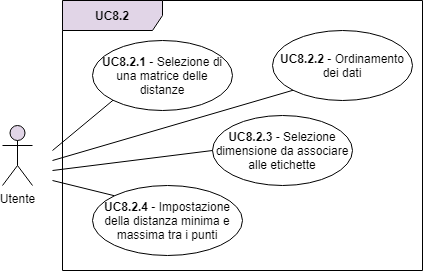
\includegraphics[width=13cm]{Section/Images/UC8.2.png}
\centering
\caption{UC8.2 - Personalizzazione Adjacency Matrix}
\end{figure}
\begin{itemize}
	\item \textbf{Attore primario}: Utente;
	
	\item \textbf{Precondizioni}: L'utente ha scelto il grafico \textit{Adjacency Matrix} [UC7.1];
	
	\item \textbf{Postcondizioni}: Il grafico viene aggiornato con le personalizzazioni impostate dall'utente.
	
	\item \textbf{Scenario principale}: L'utente decide:
	
\begin{enumerate}
\item Una matrice delle distanze calcolata in precedenza [UC8.2.1];
\item Se ordinare i dati e opzionalmente inserire il \glo{dendrogramma} [UC8.2.2];
\item Quale dimensione associare alle etichette [UC8.2.3];
\item La distanza minima e massima tra i punti per la visualizzazione [UC8.2.4];
\end{enumerate}	
		
\end{itemize}
